%||||||||||||||||||||||||||||||||||||||||||||||||||||||||||||||||||||||||||||||%
%|||||||||||||||||||||||||||||| Carga de paquetes |||||||||||||||||||||||||||||%
%||||||||||||||||||||||||||||||||||||||||||||||||||||||||||||||||||||||||||||||%

% Acá se define el tamaño de letra principal:
\documentclass[12pt]{article}

% Definición del tamaño de página y los márgenes:
\usepackage[a4paper,scale={0.80,0.80},
            headheight=15pt,headsep=20pt,voffset=15pt,footskip=50pt]{geometry}

% Vamos a escribir en castellano:
\usepackage[utf8x]{inputenc}
\usepackage[spanish]{babel}
\selectlanguage{spanish}

% El paquete amsmath agrega algunas funcionalidades extra a las fórmulas.
% Además defino la numeración de las tablas y figuras al estilo "Figura 2.3",
% en lugar de "Figura 7". (Por lo tanto, aunque no uses fórmulas, si querés
% este tipo de numeración dejá el paquete amsmath descomentado).
\usepackage{amsmath}
\numberwithin{equation}{section}
\numberwithin{figure}{section}
\numberwithin{table}{section}

% Agregado de algunos símbolos matemáticos
\usepackage{amssymb}

% Para tener cabecera y pie de página con un estilo personalizado:
\usepackage{fancyhdr}

% Para poner el texto "Figura X" en negrita:
% (Si no tenés el paquete 'caption2', probá con 'caption').
\usepackage[hang,bf]{caption}

% Para poder usar subfiguras: (al estilo Figura 2.3(b) )
%\usepackage{subfigure}

% Para poder agregar notas al pie en tablas:
%\usepackage{threeparttable}

% Para incluir imágenes, el siguiente código carga el paquete graphicx
% según se esté generando un archivo dvi o un pdf (con pdflatex).
%
% Para generar dvi, descomentá la linea siguiente:
%\usepackage[dvips]{graphicx}
%
% Para generar pdf, descomentá las dos lineas siguientes:
\usepackage[pdftex]{graphicx}
\pdfcompresslevel=9

% Directorio de imágenes:
\graphicspath{{\imgdir/}}

% Para ubicar las imágenes en un lugar específico
\usepackage{float}

% Para la utilización de colores
\usepackage[usenames,dvipsnames]{xcolor, colortbl}

% Para insertar codigo fuente (configuración en archivo externo)
% Paquete para insertar código fuente:
\usepackage{listings}

% Necesario para imprimir las comillas rectas y no las de LaTeX:
\usepackage{textcomp}

% ------------------------- Configuraciones generales ------------------------ %
\lstset
{
    extendedchars=\true,%               Incluir caracteres extendidos
    inputencoding=utf8x,%               Codificación utilizada
    linewidth=\textwidth,%              Ancho máximo de una linea de código
    xleftmargin=16pt,%                  Margen izquierdo
    xrightmargin=5pt,%                  Margen derecho
    breaklines=true,%                   Corte de lineas largas
    numbers=left,%                      Números de línea a la izquierda
    stepnumber=1,%                      Avance de los números de línea de a 1
    numbersep=5pt,%                     Separación de los números de línea
    tabsize=4,showtabs=false,%          Los TABs miden 4 espacios, y no se ven
    showstringspaces=false,%            Los espacios en las cadenas no se marcan
    upquote=true,%                      Impresión correcta de las comillas
    numberstyle=\tiny,%                 Estilo de los números de línea
    basicstyle=\ttfamily\scriptsize,%   Estilo básico del código fuente
    commentstyle=\color{Gray},%         Estilo de los comentarios
    stringstyle=\color{BrickRed},%      Estilo de las cadenas
%                 Definiciones de caracteres especiales
    literate={á}{{\'a}}1   {é}{{\'e}}1   {í}{{\'i}}1   {ó}{{\'o}}1   {ú}{{\'u}}1
             {Á}{{\'A}}1   {É}{{\'E}}1   {Í}{{\'I}}1   {Ó}{{\'O}}1   {Ú}{{\'U}}1
             {ñ}{{\~n}}1   {°}{{\textsuperscript{o}}}1
             {Ñ}{{\~N}}1   {º}{{\textsuperscript{\underline{o}}}}1
             {à}{{\`a}}1   {è}{{\`e}}1   {ì}{{\`i}}1   {ò}{{\`o}}1   {ù}{{\`u}}1
             {À}{{\`A}}1   {È}{{\`E}}1   {Ì}{{\`I}}1   {Ò}{{\`O}}1   {Ù}{{\`U}}1
}


%-------------------------- Lenguaje Assembly de AVR --------------------------%
\lstdefinelanguage{asmAVR}[x86masm]{Assembler}
{
    keywordstyle=[1]{\color{Black}},%         Estilo: en comentarios
    keywordstyle=[2]{\color{ForestGreen}},%   Estilo: definiciones de bits
    keywordstyle=[3]{\color{BurntOrange}},%   Estilo: mnemónicos
    keywordstyle=[4]{\color{MidnightBlue}},%  Estilo: definiciones de registros
    keywordstyle=[5]{\color{Violet}},%        Estilo: directivas del ensamblador
    %
    sensitive=false,%                         Case insensitive
    %
    otherkeywords=
    {TODO,XXX,FIXME,NOTE},
    %
    deletekeywords=
    {EEDR0,EEDR1,EEDR2,EEDR3,EEDR4,EEDR5,EEDR6,EEDR7,EERE,EEWE,EEMWE,EERIE,WDP0,
    WDP1,WDP2,WDE,WDTOE,WDDE,IVCE,IVSEL,INT2,INT0,INT1,INTF2,INTF0,INTF1,ISC00,
    ISC01,ISC10,ISC11,ISC2,CS00,CS01,CS02,WGM01,CTC0,COM00,COM01,WGM00,PWM0,
    FOC0,TCNT0_0,TCNT0_1,TCNT0_2,TCNT0_3,TCNT0_4,TCNT0_5,TCNT0_6,TCNT0_7,OCR0_0,
    OCR0_1,OCR0_2,OCR0_3,OCR0_4,OCR0_5,OCR0_6,OCR0_7,TOIE0,OCIE0,TOV0,OCF0,
    TOIE2,OCIE2,TOV2,OCF2,CS20,CS21,CS22,WGM21,CTC2,COM20,COM21,WGM20,PWM2,FOC2,
    TCNT2_0,TCNT2_1,TCNT2_2,TCNT2_3,TCNT2_4,TCNT2_5,TCNT2_6,TCNT2_7,OCR2_0,
    OCR2_1,OCR2_2,OCR2_3,OCR2_4,OCR2_5,OCR2_6,OCR2_7,TCR2UB,OCR2UB,TCN2UB,AS2,
    TOIE1,OCIE1B,OCIE1A,TICIE1,TOV1,OCF1B,OCF1A,ICF1,WGM10,PWM10,WGM11,PWM11,
    FOC1B,FOC1A,COM1B0,COM1B1,COM1A0,COM1A1,CS10,CS11,CS12,WGM12,CTC10,CTC1,
    WGM13,CTC11,ICES1,ICNC1,SPDR0,SPDR1,SPDR2,SPDR3,SPDR4,SPDR5,SPDR6,SPDR7,
    SPI2X,WCOL,SPIF,SPR0,SPR1,CPHA,CPOL,MSTR,DORD,SPE,SPIE,UDR0,UDR1,UDR2,UDR3,
    UDR4,UDR5,UDR6,UDR7,MPCM,U2X,UPE,PE,DOR,FE,UDRE,TXC,RXC,TXB8,RXB8,UCSZ2,
    CHR9,TXEN,RXEN,UDRIE,TXCIE,RXCIE,UCPOL,UCSZ0,UCSZ1,USBS,UPM0,UPM1,UMSEL,
    URSEL,ACME,ACIS0,ACIS1,ACIC,ACIE,ACI,ACO,ACBG,ACD,MUX0,MUX1,MUX2,MUX3,MUX4,
    ADLAR,REFS0,REFS1,ADPS0,ADPS1,ADPS2,ADIE,ADIF,ADATE,ADFR,ADSC,ADEN,ADCH0,
    ADCH1,ADCH2,ADCH3,ADCH4,ADCH5,ADCH6,ADCH7,ADCL0,ADCL1,ADCL2,ADCL3,ADCL4,
    ADCL5,ADCL6,ADCL7,ADTS0,ADTS1,ADTS2,PORTA0,PA0,PORTA1,PA1,PORTA2,PA2,PORTA3,
    PA3,PORTA4,PA4,PORTA5,PA5,PORTA6,PA6,PORTA7,PA7,DDA0,DDA1,DDA2,DDA3,DDA4,
    DDA5,DDA6,DDA7,PINA0,PINA1,PINA2,PINA3,PINA4,PINA5,PINA6,PINA7,PORTB0,PB0,
    PORTB1,PB1,PORTB2,PB2,PORTB3,PB3,PORTB4,PB4,PORTB5,PB5,PORTB6,PB6,PORTB7,
    PB7,DDB0,DDB1,DDB2,DDB3,DDB4,DDB5,DDB6,DDB7,PINB0,PINB1,PINB2,PINB3,PINB4,
    PINB5,PINB6,PINB7,PORTC0,PC0,PORTC1,PC1,PORTC2,PC2,PORTC3,PC3,PORTC4,PC4,
    PORTC5,PC5,PORTC6,PC6,PORTC7,PC7,DDC0,DDC1,DDC2,DDC3,DDC4,DDC5,DDC6,DDC7,
    PINC0,PINC1,PINC2,PINC3,PINC4,PINC5,PINC6,PINC7,PORTD0,PD0,PORTD1,PD1,
    PORTD2,PD2,PORTD3,PD3,PORTD4,PD4,PORTD5,PD5,PORTD6,PD6,PORTD7,PD7,DDD0,DDD1,
    DDD2,DDD3,DDD4,DDD5,DDD6,DDD7,PIND0,PIND1,PIND2,PIND3,PIND4,PIND5,PIND6,
    PIND7,SREG_C,SREG_Z,SREG_N,SREG_V,SREG_S,SREG_H,SREG_T,SREG_I,SM0,SM1,SM2,
    SE,PORF,EXTRF,BORF,WDRF,JTRF,JTD,CAL0,CAL1,CAL2,CAL3,CAL4,CAL5,CAL6,CAL7,
    PSR10,PSR2,PUD,SPMEN,PGERS,PGWRT,BLBSET,RWWSRE,ASRE,RWWSB,ASB,SPMIE,TWBR0,
    TWBR1,TWBR2,TWBR3,TWBR4,TWBR5,TWBR6,TWBR7,TWIE,TWEN,TWWC,TWSTO,TWSTA,TWEA,
    TWINT,TWPS0,TWPS1,TWS3,TWS4,TWS5,TWS6,TWS7,TWD0,TWD1,TWD2,TWD3,TWD4,TWD5,
    TWD6,TWD7,TWGCE,TWA0,TWA1,TWA2,TWA3,TWA4,TWA5,TWA6,LB1,LB2,BLB01,BLB02,
    BLB11,BLB12,CKSEL0,CKSEL1,CKSEL2,CKSEL3,BODEN,BODLEVEL,BOOTRST,BOOTSZ0,
    BOOTSZ1,EESAVE,SPIEN,JTAGEN,OCDEN},
    keywords=[2]
    {EEDR0,EEDR1,EEDR2,EEDR3,EEDR4,EEDR5,EEDR6,EEDR7,EERE,EEWE,EEMWE,EERIE,WDP0,
    WDP1,WDP2,WDE,WDTOE,WDDE,IVCE,IVSEL,INT2,INT0,INT1,INTF2,INTF0,INTF1,ISC00,
    ISC01,ISC10,ISC11,ISC2,CS00,CS01,CS02,WGM01,CTC0,COM00,COM01,WGM00,PWM0,
    FOC0,TCNT0_0,TCNT0_1,TCNT0_2,TCNT0_3,TCNT0_4,TCNT0_5,TCNT0_6,TCNT0_7,OCR0_0,
    OCR0_1,OCR0_2,OCR0_3,OCR0_4,OCR0_5,OCR0_6,OCR0_7,TOIE0,OCIE0,TOV0,OCF0,
    TOIE2,OCIE2,TOV2,OCF2,CS20,CS21,CS22,WGM21,CTC2,COM20,COM21,WGM20,PWM2,FOC2,
    TCNT2_0,TCNT2_1,TCNT2_2,TCNT2_3,TCNT2_4,TCNT2_5,TCNT2_6,TCNT2_7,OCR2_0,
    OCR2_1,OCR2_2,OCR2_3,OCR2_4,OCR2_5,OCR2_6,OCR2_7,TCR2UB,OCR2UB,TCN2UB,AS2,
    TOIE1,OCIE1B,OCIE1A,TICIE1,TOV1,OCF1B,OCF1A,ICF1,WGM10,PWM10,WGM11,PWM11,
    FOC1B,FOC1A,COM1B0,COM1B1,COM1A0,COM1A1,CS10,CS11,CS12,WGM12,CTC10,CTC1,
    WGM13,CTC11,ICES1,ICNC1,SPDR0,SPDR1,SPDR2,SPDR3,SPDR4,SPDR5,SPDR6,SPDR7,
    SPI2X,WCOL,SPIF,SPR0,SPR1,CPHA,CPOL,MSTR,DORD,SPE,SPIE,UDR0,UDR1,UDR2,UDR3,
    UDR4,UDR5,UDR6,UDR7,MPCM,U2X,UPE,PE,DOR,FE,UDRE,TXC,RXC,TXB8,RXB8,UCSZ2,
    CHR9,TXEN,RXEN,UDRIE,TXCIE,RXCIE,UCPOL,UCSZ0,UCSZ1,USBS,UPM0,UPM1,UMSEL,
    URSEL,ACME,ACIS0,ACIS1,ACIC,ACIE,ACI,ACO,ACBG,ACD,MUX0,MUX1,MUX2,MUX3,MUX4,
    ADLAR,REFS0,REFS1,ADPS0,ADPS1,ADPS2,ADIE,ADIF,ADATE,ADFR,ADSC,ADEN,ADCH0,
    ADCH1,ADCH2,ADCH3,ADCH4,ADCH5,ADCH6,ADCH7,ADCL0,ADCL1,ADCL2,ADCL3,ADCL4,
    ADCL5,ADCL6,ADCL7,ADTS0,ADTS1,ADTS2,PORTA0,PA0,PORTA1,PA1,PORTA2,PA2,PORTA3,
    PA3,PORTA4,PA4,PORTA5,PA5,PORTA6,PA6,PORTA7,PA7,DDA0,DDA1,DDA2,DDA3,DDA4,
    DDA5,DDA6,DDA7,PINA0,PINA1,PINA2,PINA3,PINA4,PINA5,PINA6,PINA7,PORTB0,PB0,
    PORTB1,PB1,PORTB2,PB2,PORTB3,PB3,PORTB4,PB4,PORTB5,PB5,PORTB6,PB6,PORTB7,
    PB7,DDB0,DDB1,DDB2,DDB3,DDB4,DDB5,DDB6,DDB7,PINB0,PINB1,PINB2,PINB3,PINB4,
    PINB5,PINB6,PINB7,PORTC0,PC0,PORTC1,PC1,PORTC2,PC2,PORTC3,PC3,PORTC4,PC4,
    PORTC5,PC5,PORTC6,PC6,PORTC7,PC7,DDC0,DDC1,DDC2,DDC3,DDC4,DDC5,DDC6,DDC7,
    PINC0,PINC1,PINC2,PINC3,PINC4,PINC5,PINC6,PINC7,PORTD0,PD0,PORTD1,PD1,
    PORTD2,PD2,PORTD3,PD3,PORTD4,PD4,PORTD5,PD5,PORTD6,PD6,PORTD7,PD7,DDD0,DDD1,
    DDD2,DDD3,DDD4,DDD5,DDD6,DDD7,PIND0,PIND1,PIND2,PIND3,PIND4,PIND5,PIND6,
    PIND7,SREG_C,SREG_Z,SREG_N,SREG_V,SREG_S,SREG_H,SREG_T,SREG_I,SM0,SM1,SM2,
    SE,PORF,EXTRF,BORF,WDRF,JTRF,JTD,CAL0,CAL1,CAL2,CAL3,CAL4,CAL5,CAL6,CAL7,
    PSR10,PSR2,PUD,SPMEN,PGERS,PGWRT,BLBSET,RWWSRE,ASRE,RWWSB,ASB,SPMIE,TWBR0,
    TWBR1,TWBR2,TWBR3,TWBR4,TWBR5,TWBR6,TWBR7,TWIE,TWEN,TWWC,TWSTO,TWSTA,TWEA,
    TWINT,TWPS0,TWPS1,TWS3,TWS4,TWS5,TWS6,TWS7,TWD0,TWD1,TWD2,TWD3,TWD4,TWD5,
    TWD6,TWD7,TWGCE,TWA0,TWA1,TWA2,TWA3,TWA4,TWA5,TWA6,LB1,LB2,BLB01,BLB02,
    BLB11,BLB12,CKSEL0,CKSEL1,CKSEL2,CKSEL3,BODEN,BODLEVEL,BOOTRST,BOOTSZ0,
    BOOTSZ1,EESAVE,SPIEN,JTAGEN,OCDEN},
    %
    deletekeywords=
    {adc,add,adiw,and,andi,asr,bclr,bld,brbc,brbs,brcc,brcs,break,breq,brge,
    brhc,brhs,brid,brie,brlo,brlt,brmi,brne,brpl,brsh,brtc,brts,brvc,brvs,bset,
    bst,call,cbi,cbr,clc,clh,cli,cln,clr,cls,clt,clv,clz,com,cp,cpi,cpse,dec,
    des,eicall,eijmp,elpm,eor,fmul,fmuls,fmulsu,icall,ijmp,in,inc,jmp,lac,las,
    lat,ld,ldd,ldi,lds,lpm,lsl,lsr,mov,movw,mul,muls,mulsu,neg,nop,or,ori,out,
    pop,push,rcall,ret,reti,rjmp,rol,ror,sbc,sbci,sbi,sbic,sbis,sbiw,sbr,sbrc,
    sbrs,sec,seh,sei,sen,ser,ses,set,sev,sez,sleep,spm,st,std,sts,sub,subi,swap,
    tst,wdr,xch},
    keywords=[3]
    {adc,add,adiw,and,andi,asr,bclr,bld,brbc,brbs,brcc,brcs,break,breq,brge,
    brhc,brhs,brid,brie,brlo,brlt,brmi,brne,brpl,brsh,brtc,brts,brvc,brvs,bset,
    bst,call,cbi,cbr,clc,clh,cli,cln,clr,cls,clt,clv,clz,com,cp,cpi,cpse,dec,
    des,eicall,eijmp,elpm,eor,fmul,fmuls,fmulsu,icall,ijmp,in,inc,jmp,lac,las,
    lat,ld,ldd,ldi,lds,lpm,lsl,lsr,mov,movw,mul,muls,mulsu,neg,nop,or,ori,out,
    pop,push,rcall,ret,reti,rjmp,rol,ror,sbc,sbci,sbi,sbic,sbis,sbiw,sbr,sbrc,
    sbrs,sec,seh,sei,sen,ser,ses,set,sev,sez,sleep,spm,st,std,sts,sub,subi,swap,
    tst,wdr,xch},
    %
    keywords=[4]
    {SREG,SPL,SPH,OCR0,GICR,GIFR,TIMSK,TIFR,SPMCR,TWCR,MCUCR,MCUCSR,MCUSR,TCCR0,
    TCNT0,OSCCAL,OCDR,SFIOR,TCCR1A,TCCR1B,TCNT1L,TCNT1H,OCR1AL,OCR1AH,OCR1BL,
    OCR1BH,ICR1L,ICR1H,TCCR2,TCNT2,OCR2,ASSR,WDTCR,UBRRH,UCSRC,EEARL,EEARH,EEDR,
    EECR,PORTA,DDRA,PINA,PORTB,DDRB,PINB,PORTC,DDRC,PINC,PORTD,DDRD,PIND,SPDR,
    SPSR,SPCR,UDR,UCSRA,USR,UCSRB,UCR,UBRRL,ACSR,ADMUX,ADCSRA,ADCSR,ADCH,ADCL,
    TWDR,TWAR,TWSR,TWBR,GIMSK,UBRRHI,FLASHEND,IOEND,SRAM_START,SRAM_SIZE,RAMEND,
    XRAMEND,E2END,EEPROMEND,EEADRBITS,NRWW_START_ADDR,NRWW_STOP_ADDR,
    RWW_START_ADDR,RWW_STOP_ADDR,PAGESIZE,FIRSTBOOTSTART,SECONDBOOTSTART,
    THIRDBOOTSTART,FOURTHBOOTSTART,SMALLBOOTSTART,LARGEBOOTSTART,INT0addr,
    INT1addr,INT2addr,OC2addr,OVF2addr,ICP1addr,OC1Aaddr,OC1Baddr,OVF1addr,
    OC0addr,OVF0addr,SPIaddr,URXCaddr,UDREaddr,UTXCaddr,ADCCaddr,ERDYaddr,
    ACIaddr,TWIaddr,SPMRaddr,INT_VECTORS_SIZE},
    %
    keywords=[5]
    {.byte,.cseg,.db,.def,.device,.dseg,.dw,.endmacro,.equ,.eseg,.exit,.include,
    .list,.listmac,.macro,.nolist,.org,.set,low,high,byte2,byte3,byte4,lwrd,
    hwrd,page,exp2,log2}
}


% Para utilizar hipervínculos
\usepackage{hyperref}

% Para dibujar gráficos vectoriales (también añade el bucle 'for')
\usepackage{tikz}

% Agregado de caligrafía matemática
\usepackage{bbold}

% Tablas con filas y columnas colapsadas
\usepackage{multirow}

% Unidades del SI
\usepackage{siunitx}
\sisetup{per-mode=fraction} % Fración en vez de exponente -1
\sisetup{output-decimal-marker = {,}} % Coma en vez de punto decimal
\ifx \bit \undefined % Definición de bit, si falta
    \DeclareSIUnit\bit{bit}
\fi

% Flechas largas
% \usepackage{extarrows}

% Configuración de párrafos
\usepackage{parskip}
\setlength{\parindent}{20pt}

%------------------- Datos modificables desde archivo aparte ------------------%
\newcommand\integrante[3]{
    & #1, #2 & #3 \\ \cline{2-3}
}
%||||||||||||||||||||||||||||||||||||||||||||||||||||||||||||||||||||||||||||||%
%|||||||||||||||||||||||||||||| Datos del informe |||||||||||||||||||||||||||||%
%||||||||||||||||||||||||||||||||||||||||||||||||||||||||||||||||||||||||||||||%
\newcommand\codmateria{66.09/86.07}
\newcommand\nommateria{Laboratorio de Microcomputadoras}
\newcommand\turno{1 (Martes 19 a 22 hs)}
\newcommand\docente{Stola, Gerardo}
\newcommand\autores{Cassani - Ferrari Bihurriet - Gomez}
\newcommand\anio{2015}
\newcommand\cuatrim{Segundo}
\newcommand\titulo{Corrector de impedancia}
\newcommand\fecha{\today}
\newcommand\integrantes{ % \integrante{Apellido}{Nombre}{padrón}
    \integrante{Cassani}{María Victoria}{95.145}
    \integrante{Ferrari Bihurriet}{Francisco}{92.275}
    \integrante{Gomez}{Kevin Leonel}{93.906}
}
% Descomentar para mostrar el índice
%\newcommand\indice{}
% Directorio de imágenes
\newcommand\imgdir{./img}

%------------------------------------------------------------------------------%

% Título y autor(es):
\title{\titulo}
\author{\autores}



%||||||||||||||||||||||||||||||||||||||||||||||||||||||||||||||||||||||||||||||%
%|||||||||||||||||||||||||||| Inicio del documento ||||||||||||||||||||||||||||%
%||||||||||||||||||||||||||||||||||||||||||||||||||||||||||||||||||||||||||||||%
\begin{document}

% Estilo de encabezado y pie de página:
\pagestyle{fancy}
\renewcommand{\headrule}{\vspace{-3mm}\textcolor{Gray}{\hrule}}
\renewcommand{\footrule}{\textcolor{Gray}{\hrule}\vspace{1mm}}
\lhead{\textcolor{Gray}{\textsf{\codmateria\ - \nommateria}}}
\chead{}
\rhead{\textcolor{Gray}{\textsf{\titulo}}}
\lfoot{\textcolor{Gray}{\textsf{\autores}}}
\cfoot{}
\rfoot{\textcolor{Gray}{\boxed{\textbf{\textsf{\thepage}}}}}

% Carátula:
\begin{titlepage}

    \thispagestyle{empty}

    \begin{center}

        \minipage{0.4\textwidth}
            \minipage{0.16\textwidth}
                
\includegraphics[scale=0.11]{fiuba}
            \endminipage
            \minipage{0.84\textwidth}
                \huge{\textbf{F\ i\ u\ b\ a}}\\
                \large{\textrm{Facultad de Ingeniería}}\\
                \normalsize{\textrm{Universidad de Buenos Aires}}
            \endminipage
        \endminipage
        \minipage{0.6\textwidth}
            \begin{center}
                \large{\textsc{\nommateria\\(\codmateria)}}
            \end{center}
        \endminipage

        \vfill

        \hrule
        \large{\textsc{Informe Final del Proyecto}}
        \vspace{2mm}\hrule

        \vfill

        \begin{tabular}{|p{0.3\textwidth}|p{0.4\textwidth}|p{0.2\textwidth}|}
            \hline
            \textbf{Proyecto:} &
                \multicolumn{2}{p{0.6\textwidth}|}{\textbf{\titulo}}\\[6pt]
            \hline
            Autores: \integrantes
            \hline
            Turno de TP: &
                \multicolumn{2}{p{0.6\textwidth}|}{\turno}\\
            \hline
            Año y Cuatrimestre: & \anio & \cuatrim \\
            \hline
            Docente Guía: &
                \multicolumn{2}{p{0.6\textwidth}|}{\docente}\\
            \hline
        \end{tabular}

        \vfill

        \begin{tabular}{|p{0.95\textwidth}|}
            \hline \vfill
            Observaciones Generales
            \\[6pt] \hline
            \\[12pt] \hline
            \\[12pt] \hline
            \\[12pt] \hline
            \\[12pt] \hline
            \\[12pt] \hline
            \\[12pt] \hline
            \\[12pt] \hline
        \end{tabular}

        \vfill

        \begin{tabular}{|p{0.314\textwidth}|p{0.61\textwidth}|}
            \hline
            \vfill Calificación Final \vfill & \\[36pt]
            \hline
            \vfill Firma del Docente \vfill & \\[36pt]
            \hline
            \vfill Fecha \vfill & \\[6pt]
            \hline
        \end{tabular}

    \end{center}

\end{titlepage}

% Hago que las páginas se comiencen a contar desde aquí
\setcounter{page}{1}

% Pongo el índice en una página aparte:
\ifx \indice \undefined
\else
    \tableofcontents
    \newpage
\fi



%||||||||||||||||||||||||||||||||||||||||||||||||||||||||||||||||||||||||||||||%
%||||||||||||||||||||||||| Definiciones para abreviado ||||||||||||||||||||||||%
%||||||||||||||||||||||||||||||||||||||||||||||||||||||||||||||||||||||||||||||%

% Gráficos comunes:
% \figuregraph{escala}{nombre/etiqueta}{pie de imagen}
\newcommand{\figuregraph}[3]{
    \begin{figure}[H]
        \center
        \includegraphics[scale=#1]{#2}
        \caption{#3}\label{#2}
    \end{figure}
}

% Dos gráficos horizontales:
% \twofigures{escala1}{nombre/etiqueta1}{pie1}{escala2}{nombre/etiqueta2}{pie2}
\newcommand{\twofigures}[6]{
    \begin{figure}[H]
        \minipage{0.5\textwidth}
            \center
            \includegraphics[scale=#1]{#2}
            \caption{#3}\label{#2}
        \endminipage
        \minipage{0.5\textwidth}
            \center
            \includegraphics[scale=#4]{#5}
            \caption{#6}\label{#5}
        \endminipage
    \end{figure}
}


%------------------- Cuerpo del documento en archivo aparte -------------------%
%|//////////////////////////////////////|\\\\\\\\\\\\\\\\\\\\\\\\\\\\\\\\\\\\\|%
%|//////////////////////////| Objetivo del Proyecto |\\\\\\\\\\\\\\\\\\\\\\\\\|%
%|//////////////////////////////////////|\\\\\\\\\\\\\\\\\\\\\\\\\\\\\\\\\\\\\|%
\section{Objetivo del Proyecto}
% El objetivo es la respuesta a la pregunta “¿para qué?”; tiene que satisfacer alguna necesidad del usuario.

El presente proyecto consiste en el diseño y desarrollo de un sistema de calibración de impedancia y ajuste por electrodeposición (galvanoplastía). Este instrumento se utilizará en el futuro en aplicaciones biomédicas, más precisamente en la fabricación de electrodos de registro extracelular.



%|//////////////////////////////////////|\\\\\\\\\\\\\\\\\\\\\\\\\\\\\\\\\\\\\|%
%|////////////////////////| Descripción del Proyecto |\\\\\\\\\\\\\\\\\\\\\\\\|%
%|//////////////////////////////////////|\\\\\\\\\\\\\\\\\\\\\\\\\\\\\\\\\\\\\|%
\section{Descripción del Proyecto}
% En esta sección se responde la pregunta “¿cómo?”. Aquí se enumeran las prestaciones, las funciones y el comportamiento o uso del equipo.
El equipo consiste en un circuito con un microcontrolador que genera señales senoidales y continuas para medir y corregir las impedancias, respectivamente. Incluye una cuba conductora, que contiene una solución acuosa donde se colocan los electrodos. Éstos son similares a un filamento de cobre recubierto con esmalte aislante en su totalidad, excepto en los extremos, los cuales uno va sumergido en la solución y el otro conectado al equipo por medio de un conector especial.

El sistema funciona con 1, 4, 8, 12 ó 16 electrodos, corrigiendo de a uno por vez. El usuario coloca los electrodos procurando que no se produzcan cortocircuitos entre los mismos (se debería detectar esto antes de comenzar). Hay tres opciones: medir, calibrar y corregir. La primera permite ver el/los valor/es de la/s impedancia/s colocada/s en los conectores. La segunda, calibrar el equipo tal como su nombre lo indica. La opción de corregir permite que el usuario seleccione la impedancia final deseada, el tiempo máximo de espera para la corrección y dé la orden de inicio. Luego de algunos chequeos básicos se da comienzo al proceso. Al terminar con todos los electrodos, se muestra la impedancia final de cada uno. 

En líneas generales, el sistema consta de módulos de amplificación y filtros de PWM que permiten generar una señal senoidal con el microcontrolador, además de controlar la señal de offset. Asimismo, hay una fuente de corriente controlada por tensión que permite inyectar corriente continua al sistema para poder disminuir las impedancias necesarias por galvanoplastía. 

La señal de salida del PWM es una corriente senoidal de \SI{1}{\kilo\hertz}, con uno de los siguientes valores de amplitud: $\{\SI{30}{\nano\ampere}, \SI{80}{\nano\ampere}, \SI{120}{\nano\ampere}, \SI{200}{\nano\ampere}\}$. Éstos se seleccionan con un multiplexor dependiendo del rango de impedancias: $\{0-\SI{2}{\mega\ohm}, 0-\SI{8}{\mega\ohm}, 0-\SI{20}{\mega\ohm}, 0-\SI{60}{\mega\ohm}\}$. Considerando la ley de Ohm y midiendo el valor pico de tensión, se calcula la impedancia del electrodo en estudio como $Z@\SI{1}{\kilo\hertz} = \frac{\hat{v}}{\hat{\i}}$. Este valor se puede disminuir porque la solución acuosa contiene oro o plata, de modo de que se produce un recubrimiento por galvanoplastía sobre el electrodo y así disminuye la impedancia. Si este proceso es necesario o no, dependerá del resultado previo y de la comparación entre el valor obtenido en la medición y el de referencia establecido previamente por el usuario. Se emplea un multiplexor analógico para ir seleccionando cada electrodo y otro en paralelo con éste, que será eventualmente utilizado para verificar que no haya cortocircuitos entre electrodos (inyectando señal en cada electrodo y chequeando sobre cada uno de los restantes que no se reciba un nivel elevado de ésta). 

Cada \SI{1}{\minute}) se mide la impedancia y se corrige de ser necesario. Este proceso se repite tantas veces como se requiera hasta llegar al valor de impedancia deseada determinado previamente en la configuración. Los valores aceptables para empezar el proceso están entre \SI{1}{\mega\ohm} y \SI{8}{\mega\ohm}. Además, hay que pautar un tiempo máximo de sensado y corrección, para que el sistema deje de actuar en caso de haber pasado ese tiempo sin haber llegado al valor buscado. Éste puede valer 10, 20, 30, 40, 50 ó 60 minutos.

%|//////////////////////////////////////|\\\\\\\\\\\\\\\\\\\\\\\\\\\\\\\\\\\\\|%
%|/////////////////////////| Periféricos Principales |\\\\\\\\\\\\\\\\\\\\\\\\|%
%|//////////////////////////////////////|\\\\\\\\\\\\\\\\\\\\\\\\\\\\\\\\\\\\\|%

% Los periféricos son los elementos ajenos al microcontrolador con los que interactúa el equipo y deben estar claramente definidos (por ejemplo: motores, display, teclado, puertos de comunicación, sensores, etc.)

El dispositivo tiene una pantalla LCD donde se muestran las opciones de configuración para seleccionar a través de un menú y también los resultados del proceso, además de los mensajes de error o alerta (en caso de ocurrir algún imprevisto o no llegar al valor deseado en el tiempo pautado, por ejemplo). Las opciones se seleccionan desde un teclado de 4 botones (\texttt{ok}, \texttt{cancelar}, \texttt{mover izquierda}, \texttt{mover derecha}).

Además, como periféricos principales están los circuitos mencionados antes, a través de los cuales se interactúa directamente con los electrodos. Asimismo, otros elementos importantes con los que interactúa el microcontrolador son los multiplexores, que tienen 2 ó 4 entradas de control, según sean de 4 canales o 16, y la cuba electrolítica donde se produce la reacción química para disminuir la impedancia, que está compuesta por un material conductor, el cual también debe conectarse.


%|//////////////////////////////////////|\\\\\\\\\\\\\\\\\\\\\\\\\\\\\\\\\\\\\|%
%|///////////////| Características y Especificaciones Mínimas |\\\\\\\\\\\\\\\|%
%|//////////////////////////////////////|\\\\\\\\\\\\\\\\\\\\\\\\\\\\\\\\\\\\\|%

% Las especificaciones acotan las bondades del equipo. Deben listarse los rangos de funcionamiento o requerimientos externos (por ejemplo: tensión de alimentación, consumo, temperatura de funcionamiento, protocolos de comunicaciones, rangos de medición, etc.)

Las especificaciones del sistema son:

\begin{table}[H]
\begin{center}
\begin{tabular}{|r|l|}
    \hline
    Tensión de alimentación &
    \SI{5}{\volt} \\ \hline
    Consumo &
    $<$ \SI{500}{\milli\ampere} (\SI{2.5}{\watt}) \\ \hline
    Temperatura de funcionamiento &
    \SI{5}{\celsius} - \SI{70}{\celsius} \\ \hline
    Rango de impedancias de los electrodos medidos &
    \SI{0}{\mega\ohm} - \SI{60}{\mega\ohm} (@ \SI{1}{\kilo\hertz})\\ \hline
    Impedancia buscada & $\simeq$ \SI{1}{\mega\ohm}\\ \hline
    Cantidad de electrodos a conectar &
    1, 4, 8, 12 ó 16 \\ \hline
    Tiempo máximo de corrección por electrodo &
    \SI{90}{\minute} (*)\\ \hline
    Modo medición & señal senoidal, \SI{1}{\kilo\hertz}, error $<$ 10 \% \\ \hline
    Modo corrección & señal continua 30/80/120/\SI{200}{\nano\ampere}, error $<$ 20\% \\ \hline
\end{tabular}
\end{center}
\end{table}

(*) una vez cumplido este tiempo se abandonan los esfuerzos.



%|//////////////////////////////////////|\\\\\\\\\\\\\\\\\\\\\\\\\\\\\\\\\\\\\|%
%|/////////////////////| Diagrama en Bloques (hardware) |\\\\\\\\\\\\\\\\\\\\\|%
%|//////////////////////////////////////|\\\\\\\\\\\\\\\\\\\\\\\\\\\\\\\\\\\\\|%
\pagebreak
\section{Diagrama en Bloques (hardware)}
% El esquema general de interconexión de todos los dispositivos importantes se representa mediante un diagrama en bloques.
El diagrama de bloques aquí abajo muestra la interconexión de los dispositivos más relevantes del sistema.
\begin{center}
    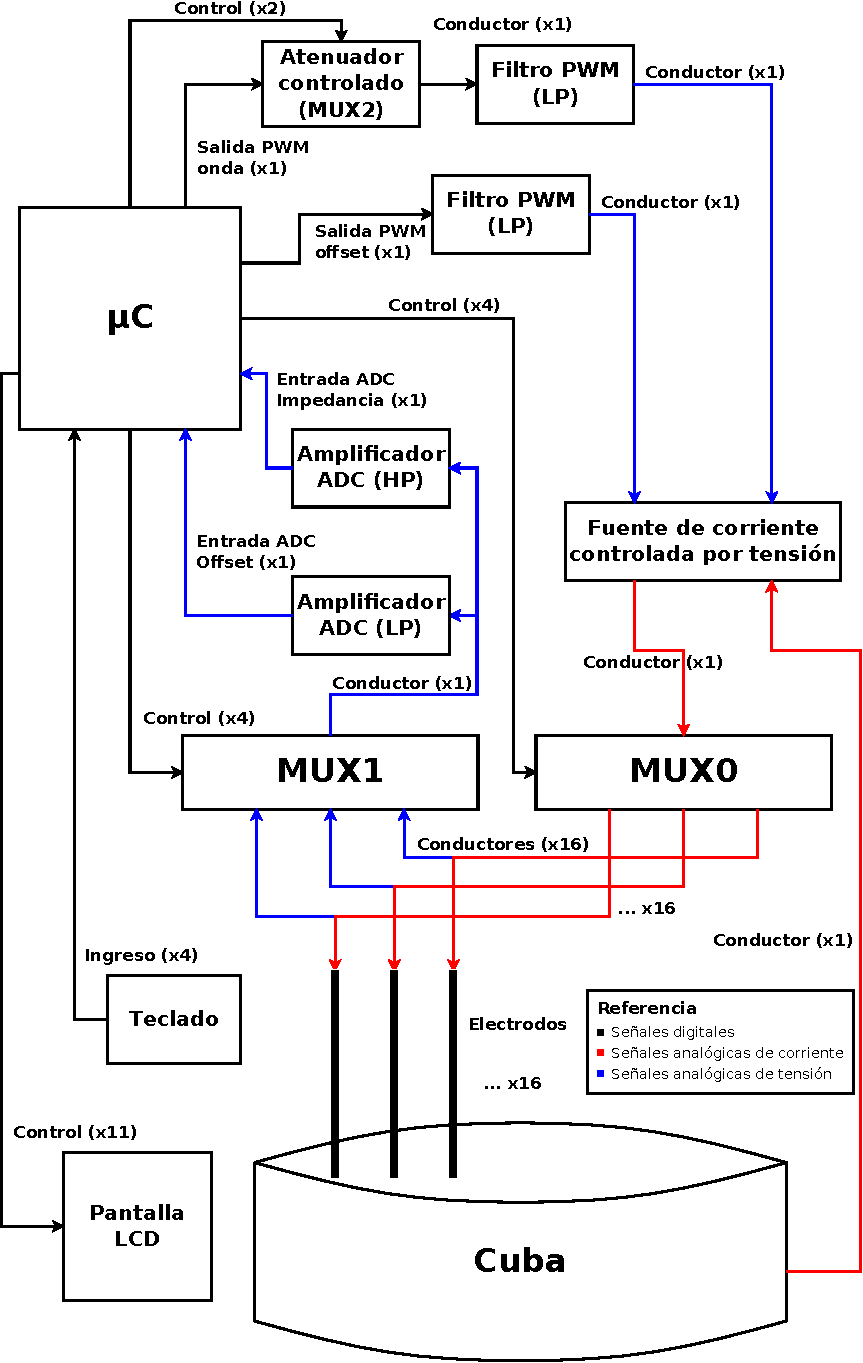
\includegraphics[scale=0.9]{bloques}
\end{center}



%|//////////////////////////////////////|\\\\\\\\\\\\\\\\\\\\\\\\\\\\\\\\\\\\\|%
%|//////////////////////| Diagrama de Flujo (firmware) |\\\\\\\\\\\\\\\\\\\\\\|%
%|//////////////////////////////////////|\\\\\\\\\\\\\\\\\\\\\\\\\\\\\\\\\\\\\|%
\section{Diagrama de Flujo  (firmware)}
% El diagrama de flujo ilustra de manera general la interacción entre los distintos bloques (o rutinas) de código.
El diagrama de flujo final del proyecto es el siguiente:
\begin{center}
    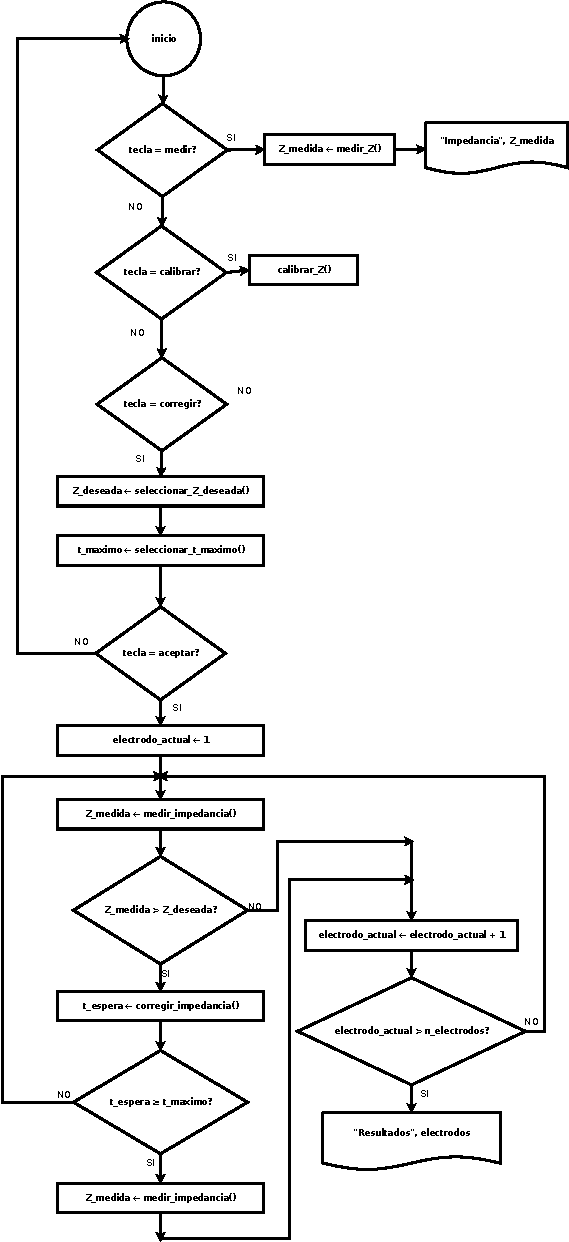
\includegraphics[scale=1.1]{flujo}
\end{center}



%|//////////////////////////////////////|\\\\\\\\\\\\\\\\\\\\\\\\\\\\\\\\\\\\\|%
%|//////////////////////////| Circuito Esquemático |\\\\\\\\\\\\\\\\\\\\\\\\\\|%
%|//////////////////////////////////////|\\\\\\\\\\\\\\\\\\\\\\\\\\\\\\\\\\\\\|%
\section{Circuito Esquemático}
% La representación del circuito eléctrico final del prototipo debe realizarse en algún sistema CAD; no es necesario el diseño del circuito impreso (PCB), basta con el circuito esquemático.
A continuación se muestra el circuito esquemático correspondiente al prototipo, así como también el diseño del PCB. Ambos fueron realizados con el programa KiCad.\\
 
\hspace{-1.8cm}
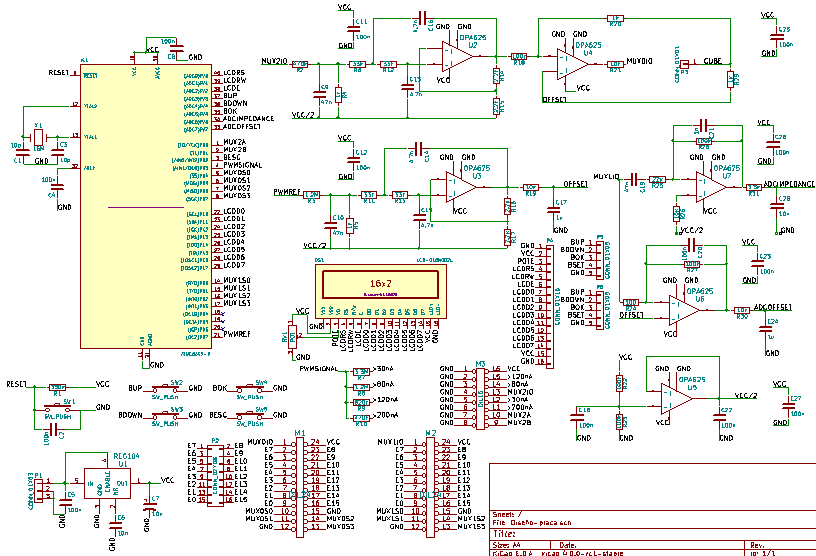
\includegraphics[scale=0.7]{circuito_esquematico}



%|//////////////////////////////////////|\\\\\\\\\\\\\\\\\\\\\\\\\\\\\\\\\\\\\|%
%|////////////////| Listado de Componentes y Costos Estimados |\\\\\\\\\\\\\\\|%
%|//////////////////////////////////////|\\\\\\\\\\\\\\\\\\\\\\\\\\\\\\\\\\\\\|%
\pagebreak
\section{Listado de Componentes y Costos}
% En esta sección se debe incluir el listado final de componentes con sus respectivos costos. Además deben incorporar la estimación de horas-hombre insumidas en la realización del proyecto. 
Los componentes que se emplearon para la construcción del dispositivo se muestran en la tabla siguiente:

\begin{table}[H]
\begin{center}
\begin{tabular}{|l|rr|}
    \hline
    \textbf{Componente} & \multicolumn{2}{c|}{\textbf{Costo}} \\ \hline
    Atmega32            & \hspace{2.8cm}\$ &   164.5 \\ \hline
    OPA625 x6 (*)       & \$               &   166.2 \\ \hline
    REG104 (*)          & \$               &   70.0 \\ \hline
    CD74HC4067 x2 (*)   & \$               &   16.8 \\ \hline
    SN74LV4052 (*)      & \$               &   5.0 \\ \hline
    Resistencias x30    & \$               &   9.6 \\ \hline
    Potenciómetro       & \$               &   6.7 \\ \hline
    Capacitores x31     & \$               &   43.1 \\ \hline
    Display LCD         & \$               &   120.0 \\ \hline
    Pulsadores x5       & \$               &   18.8 \\ \hline
    Cristal 16 Mhz      & \$               &   6.0 \\ \hline 
    Conectores          & \$               &   8.6 \\ \hline       
    Placa Epoxy         & \$               &   120.0 \\ \hline
    Zócalo              & \$               &   3.0 \\ \hline
    Jack power          & \$               &   3.2 \\ \hline           
    TOTAL               & \$               &   761.5 \\ \hline
\end{tabular}
\end{center}
\end{table}

Los componentes marcados con un asterisco(*) son de Texas Instruments y en el marco del IIBM y de la Facultad se obtuvieron como muestras gratis. Por ende, para este trabajo en particular el costo de los componentes utilizados fue de $\$ 503.5$.\\

En cuanto a las horas-hombre involucradas, se puede estimar un número de 200 horas/hombre. 



%|//////////////////////////////////////|\\\\\\\\\\\\\\\\\\\\\\\\\\\\\\\\\\\\\|%
%|///////////////////////////////| Resultados |\\\\\\\\\\\\\\\\\\\\\\\\\\\\\\\|%
%|//////////////////////////////////////|\\\\\\\\\\\\\\\\\\\\\\\\\\\\\\\\\\\\\|%
\section{Resultados}
% No siempre se logran los objetivos propuestos (o al menos en su totalidad); es importante que puedan validar y/o ajustar las expectativas indicando las limitaciones finales del prototipo construido.



%|//////////////////////////////////////|\\\\\\\\\\\\\\\\\\\\\\\\\\\\\\\\\\\\\|%
%|//////////////////////////////| Conclusiones |\\\\\\\\\\\\\\\\\\\\\\\\\\\\\\|%
%|//////////////////////////////////////|\\\\\\\\\\\\\\\\\\\\\\\\\\\\\\\\\\\\\|%
\section{Conclusiones}
% En este punto tienen que describir mejoras posibles que podrían hacerse al equipo, cambios sugeridos en función de las experiencias aprendidas  y cualquier otra sugerencia relacionada con el proyecto.



%|//////////////////////////////////////|\\\\\\\\\\\\\\\\\\\\\\\\\\\\\\\\\\\\\|%
%|////////////////////////////////| Apéndices |\\\\\\\\\\\\\\\\\\\\\\\\\\\\\\\|%
%|//////////////////////////////////////|\\\\\\\\\\\\\\\\\\\\\\\\\\\\\\\\\\\\\|%
\section{Apéndices}
% Como complemento al informe, en esta sección deben agregar el listado completo de software, las hojas de datos principales y cualquier otra información, referencia o cálculo relacionada con el proyecto (por ejemplo el uso de interrupciones).

\subsection{Cálculos}
A continuación se muestran los cálculos involucrados en la obtención de los parámetros $p$ por el que habrá que multiplicar a la medición del valor pico para obtener la impedancia. Vale aclarar que estos son valores iniciales y luego serán corregidos durante la calibración automática del equipo.

\hspace{-1cm}
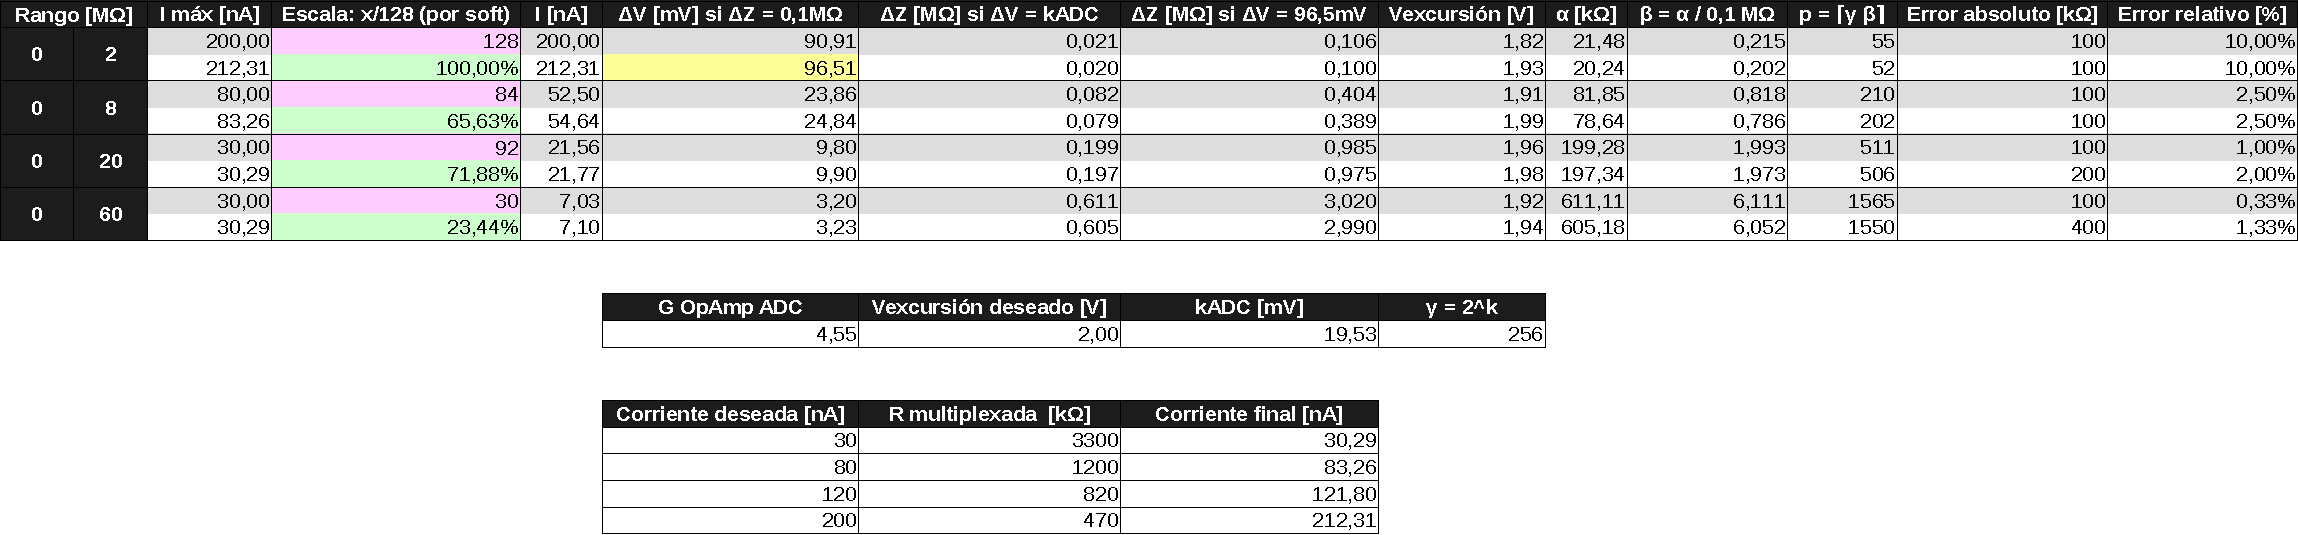
\includegraphics[scale=0.45]{calculos}

\subsection{Hojas de datos}

Los componentes empleados son:
%\begin{table}[H]
%\begin{center}
%\begin{tabular}{|l|c|}
%    \hline
%    \textbf{Componente} & \textbf{Hoja de datos}
%    \hline
%    Atmega32     & http://www.atmel.com/images/doc2503.pdf \\ \hline
%    OPA625       &  http://www.ti.com/lit/ds/symlink/opa625.pdf \\ \hline
%    REG104       &  http://www.ti.com/lit/ds/symlink/reg104.pdf \\ \hline
%    CD74HC4067   &  http://www.ti.com/lit/ds/symlink/cd74hc4067.pdf \\ \hline
%    SN74LV4052   & http://www.ti.com/lit/ds/symlink/sn74lv4052a.pdf \\ \hline
%    Display LCD  &  http://elmicro.com/files/lcd/gdm1602a_datasheet.pdf \\ \hline
%\end{tabular}
%\end{center}
%\end{table}

\begin{table}[H]
\begin{center}
\begin{tabular}{|l|c|}
    \hline
    \textbf{Componente} & \textbf{Hoja de datos} \\ \hline
    Atmega32      & \url{http://www.atmel.com/images/doc2503.pdf} \\ \hline
    OPA625        & \url{http://www.ti.com/lit/ds/symlink/opa625.pdf} \\ \hline
    REG104        & \url{http://www.ti.com/lit/ds/symlink/reg104.pdf} \\ \hline
    CD74HC4067    & \url{http://www.ti.com/lit/ds/symlink/cd74hc4067.pdf} \\ \hline
    SN74LV4052    & \url{http://www.ti.com/lit/ds/symlink/sn74lv4052a.pdf} \\ \hline
    Display LCD   & \url{http://elmicro.com/files/lcd/gdm1602a\_datasheet.pdf} \\ \hline        
\end{tabular}
\end{center}
\end{table}



\subsection{Códigos fuente}
En las siguientes páginas se incluyen a modo de apéndice todos los archivos que conforman el firmware de equipo.

%------------------------------------------------------------------------------%

\end{document} % Fin!
%%%%%%%%%%%%%%%%%%%%%%%%%%%%%%%%%%%%%%%%%%%%%%%%%%%%%%%%%%%%%%%%%%%%%%%%%%%%%%%%
